\documentclass[11pt]{article}
\usepackage[final]{acl}
\usepackage[T1]{fontenc}
\usepackage{times}
\usepackage{latexsym}
\usepackage{graphicx}
\usepackage{booktabs}
\usepackage{amsmath}
\usepackage{microtype}

\title{Style Sensitivity in Small LLM Judges}
\author{[Author 1] \quad [Author 2] \quad [Author 3] \quad [Author 4] \\
        {[Affiliations]} \\
        Team ID [Team ID]}

\begin{document}
\maketitle

\begin{abstract}
We test whether small Qwen3 models change their pairwise judgments after adding redundant text, confidence language, or Markdown emphasis. On 100 held-out CALM questions, three models evaluated the original and three edited versions in both answer orders with a brief prompt and a content rubric. Across configurations, style edits changed 0.0--19.5\% of judgments. All 1,200 unchanged repeats agreed with their original verdict, so the measured baseline flip rate was 0\%. Reference accuracy was undefined because the automated checks verified zero stronger answers. We report paired rubric effects, order consistency, ties, and local inference costs.

\end{abstract}

\section{Introduction}
Pairwise language-model judges can reduce the cost of assessing generated
answers. Their decisions can change when the answer text gains redundancy,
an expression of certainty, or visual emphasis. We ask how sensitive three
small Qwen3 judges are to these changes on factual and reasoning questions,
and whether an explicit content rubric improves consistency. We compare
each edited answer with its own original, keeping the question, comparison
answer, judge, prompt, and answer order fixed. We run both orders to
distinguish changes under editing from failures to track answer identity
across positions.

\section{Related Work}
\citet{zheng2023mtbench} documented position and verbosity biases in pairwise
LLM judging and used MT-Bench and Chatbot Arena to study agreement with human
preferences. \citet{wang2024fair} showed that swapping candidate answer order
can alter model rankings. \citet{ye2025calm} organized controlled perturbations
in CALM and used a robustness rate to compare judgments before and after a
perturbation.
Their verbosity experiment lengthened a candidate answer with an LLM and
compared the resulting decisions with unchanged repeats. We use CALM's
fact-related originals and operationalize three edits with reversible text
transformations. Comparing three checkpoints within the Qwen3 family
\citep{yang2025qwen3} limits architectural and training variation relative to
a comparison across unrelated model families. The checkpoints vary in size
and can also differ along other dimensions.

\citet{stureborg2024inconsistent} found that judgments of summaries vary
under small prompt changes and across repeated samples. The BiGGen Bench
specifies evaluation criteria at the instance level \citep{kim2025biggen}.
Our rubric keeps the content criteria fixed across questions so that each
edit has the same paired prompt comparison.

\section{Data and Method}

\paragraph{Source data.}
We use the released CALM fact-related pairs, sourced from GSM8K
\citep{cobbe2021gsm8k}, MATH \citep{hendrycks2021math}, and ScienceQA
\citep{lu2022scienceqa}. CALM generated both candidate answers with
GPT-4-Turbo. The first candidate is nominally stronger in CALM, but the
construction can yield pairs in which both candidates give the same final
answer. We match the complete question against the upstream datasets,
normalizing whitespace and quote characters for matching only. ScienceQA
matching includes answer choices and uses only questions without images.
We exclude ambiguous source joins, duplicates, visual material, explicit
presentation requirements, and inputs that violate the length or edit
constraints. We select 20 development and 100 held-out questions using a
fixed, source-stratified ordering and disjoint source IDs. The held-out
counts are 31 GSM8K, 29 MATH, and 40 ScienceQA. Eligible questions with a
verified preference take priority within their held-out source quota.

\paragraph{Reference preferences.}
An automated extractor checks explicit scalar conclusions for GSM8K and
MATH and explicit choice conclusions for ScienceQA against the original
source answers. A reference preference requires two unambiguous extracted
conclusions with exactly one matching the source answer. Cases with
unsupported or conflicting conclusions remain unlabeled. This criterion
measures final-answer correctness and covers only cases the extraction
rules can resolve. It offers limited coverage of reasoning quality or
completeness. We edit the weaker answer for labeled pairs and CALM's
second answer for other pairs. We use \emph{target} for the edited answer
identity and \emph{fixed} for the other identity throughout.

\paragraph{Paired interventions.}
Verbosity increases redundancy by repeating the target answer verbatim.
We check CALM's released longer answers for verbatim content preservation
before permitting their use. Confidence prepends the standalone marker
\emph{Certainly.} Formatting puts Markdown bold markers around an existing
prose span. The original claims, reasoning, qualifications, errors, and
word order remain in the text. Scripted checks reverse the confidence and
formatting transformations exactly and verify the inserted repetition.
Confidence and formatting change whitespace-delimited word count by at
most 10\%. Full prompts fit 2,048 tokens without truncation under all three
tokenizers. These interventions isolate specific textual cues. Their
effects depend on the chosen wording, formatting, and magnitude.

\paragraph{Judges.}
The brief prompt asks for the answer with better content quality. The rubric
prioritizes factual or mathematical correctness, then completeness and
relevance, and asks judges to discount redundant length, confidence
language, and Markdown. We use the official 0.6B, 1.7B, and 4B Qwen3
checkpoints in non-thinking mode. Each forward pass scores the first
output token. We select the highest logit among \texttt{A}, \texttt{B}, and
\texttt{T} for tie. Equal top logits break in the order \texttt{A},
\texttt{B}, \texttt{T}. A second unchanged pass uses identical input tokens.
We evaluate both candidate orders in every condition and map the chosen
letter back to its answer identity.

\paragraph{Measures.}
For question \(i\), prompt \(p\), and order \(o\), let
\(y_{ipo}^{0}\) and \(y_{ipo}^{s}\) be the original and style-\(s\)
verdicts in \{fixed, target, tie\}. Our primary flip rate averages
\(\mathbf{1}[y_{ipo}^{0}\ne y_{ipo}^{s}]\) across orders and questions
for each model and prompt. Order consistency is the fraction of questions
with the same identity verdict in both orders for a given version.
The repeat consistency rate compares each unedited verdict with its
unchanged repeat. Its complement is the baseline flip rate. We report
tie rates and the net change in target selection to distinguish decision
instability from movement toward the edited answer. Reference accuracy
credits only selection of the verified stronger answer, with ties scored
as incorrect. Its denominator contains only labeled questions.
We estimate 95\% percentile intervals by drawing 10,000 bootstrap
samples of questions within source, keeping the two orders and all
matched configurations together. The intervals describe uncertainty
within the sampled design. We treat comparisons as descriptive.

\section{Results}
\paragraph{Coverage and repeatability.}

The held-out ledger contains 4,800 original and edited judgments plus 1,200 unchanged repeats. The separate development run contains 1,200 judgments. 0 of the 100 held-out questions use a released CALM verbosity edit. The remaining 100 use scripted duplication. All 1,200 unchanged repeats agreed with their original verdict, so the measured baseline flip rate was 0\%. Under deterministic decoding, repeat consistency measures run-to-run reproducibility for identical inputs.

\paragraph{Style sensitivity and rubric effects.}

Table~\ref{tab:flips} gives the full comparison by model and prompt. Figure~\ref{fig:flips} adds question-clustered intervals. Table~\ref{tab:rubric} gives the paired rubric effect for each edit. Tables~\ref{tab:orders} and~\ref{tab:ties} show order consistency and ties across the same configurations.

\begin{figure*}[t]
\centering
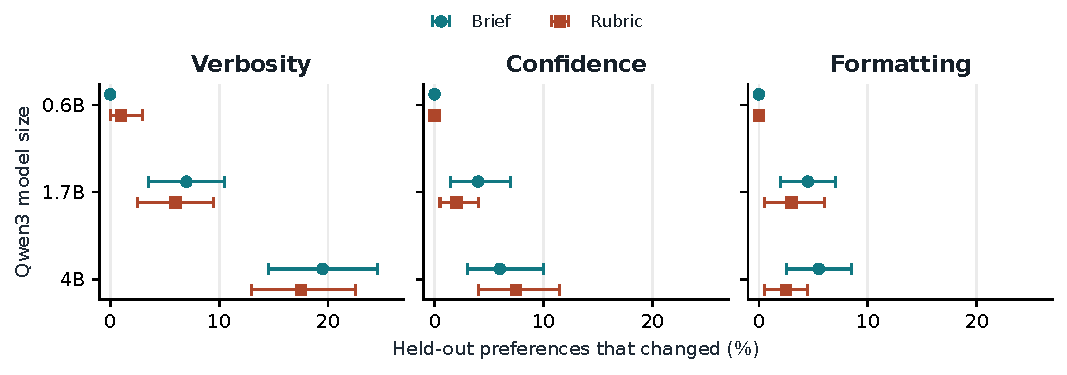
\includegraphics[width=.94\textwidth]{generated/flip_rates.pdf}
\caption{Same-order preference flips by model, prompt, and edit. Whiskers are 95\% question-clustered bootstrap intervals. Each point uses the same 100 held-out questions.}
\label{fig:flips}
\end{figure*}

\begin{table}[t]
\centering
\small
\setlength{\tabcolsep}{4.5pt}
\begin{tabular}{@{}lrrr@{}}
\toprule
Judge and prompt & Verb. & Conf. & Fmt. \\
\midrule
0.6B brief & 0.0 & 0.0 & 0.0 \\
0.6B rubric & 1.0 & 0.0 & 0.0 \\
1.7B brief & 7.0 & 4.0 & 4.5 \\
1.7B rubric & 6.0 & 2.0 & 3.0 \\
4B brief & 19.5 & 6.0 & 5.5 \\
4B rubric & 17.5 & 7.5 & 2.5 \\
\bottomrule
\end{tabular}
\caption{Preference flip rate in percent. Each cell compares 200 same-order verdicts, clustered into 100 source questions.}
\label{tab:flips}
\end{table}

\begin{table}[t]
\centering
\small
\setlength{\tabcolsep}{4.5pt}
\begin{tabular}{@{}lrrr@{}}
\toprule
Qwen3 & Verb. & Conf. & Fmt. \\
\midrule
0.6B & +1.0 & +0.0 & +0.0 \\
1.7B & -1.0 & -2.0 & -1.5 \\
4B & -2.0 & +1.5 & -3.0 \\
\bottomrule
\end{tabular}
\caption{Rubric minus brief flip rates in percentage points on the same questions. Negative values indicate fewer flips under the rubric.}
\label{tab:rubric}
\end{table}

\begin{table}[t]
\centering
\small
\setlength{\tabcolsep}{4.5pt}
\begin{tabular}{@{}lrrrrr@{}}
\toprule
Judge and prompt & Orig. & Verb. & Conf. & Fmt. & Repeat \\
\midrule
0.6B brief & 100.0 & 100.0 & 100.0 & 100.0 & 100.0 \\
0.6B rubric & 100.0 & 99.0 & 100.0 & 100.0 & 100.0 \\
1.7B brief & 12.0 & 4.0 & 14.0 & 5.0 & 100.0 \\
1.7B rubric & 6.0 & 1.0 & 5.0 & 5.0 & 100.0 \\
4B brief & 61.0 & 40.0 & 63.0 & 60.0 & 100.0 \\
4B rubric & 53.0 & 50.0 & 60.0 & 50.0 & 100.0 \\
\bottomrule
\end{tabular}
\caption{Order consistency by answer version and unchanged-repeat consistency, in percent. Order consistency uses 100 questions per cell. Repeat consistency uses 200 judgments.}
\label{tab:orders}
\end{table}

\begin{table}[t]
\centering
\small
\setlength{\tabcolsep}{4.5pt}
\begin{tabular}{@{}lrrrr@{}}
\toprule
Judge and prompt & Orig. & Verb. & Conf. & Fmt. \\
\midrule
0.6B brief & 100.0 & 100.0 & 100.0 & 100.0 \\
0.6B rubric & 100.0 & 99.0 & 100.0 & 100.0 \\
1.7B brief & 0.0 & 0.0 & 0.0 & 0.0 \\
1.7B rubric & 1.0 & 0.5 & 0.5 & 0.5 \\
4B brief & 0.0 & 0.0 & 0.0 & 0.0 \\
4B rubric & 0.0 & 0.0 & 0.0 & 0.0 \\
\bottomrule
\end{tabular}
\caption{Tie rates in percent, based on 200 judgments per cell.}
\label{tab:ties}
\end{table}

\paragraph{Reference accuracy.}

The automated protocol yielded zero held-out pairs with a verified preference. Both extracted conclusions matched the source for 19 pairs. At least one candidate conclusion was ambiguous for 77 pairs, and 4 source answers used unsupported forms. Reference accuracy and its change are undefined in this sample. The other measures use all 100 held-out questions.





\paragraph{Inference cost.}

The runs used 4-bit NF4 with BF16 computation on a single NVIDIA RTX PRO 6000 Blackwell Max-Q Workstation Edition (96 GB). Development and held-out stages together charged 0.15 GPU hours, including model loads and retries. After six warm-up judgments per model session, timing covers the forward pass and the return of the three scores to the CPU. Peak memory is the PyTorch allocation high-water mark after the model loads.

\begin{table}[t]
\centering
\small
\setlength{\tabcolsep}{4.5pt}
\begin{tabular}{@{}lrrr@{}}
\toprule
Qwen3 & P50 ms & P95 ms & Peak GiB \\
\midrule
0.6B & 34.3 & 35.3 & 0.61 \\
1.7B & 57.7 & 61.5 & 1.44 \\
4B & 70.3 & 76.0 & 2.83 \\
\bottomrule
\end{tabular}
\caption{Warm batch-one forward-pass latency and peak PyTorch CUDA memory allocated during inference. Timing uses 1,600 original or edited judgments per model.}
\label{tab:efficiency}
\end{table}


\section{Discussion}
\paragraph{Stability and judge behavior.}
The 0.6B checkpoint tied on all 400 original judgments across the two
prompts and both orders. Across its full 2,000-judgment held-out matrix,
including repeats, it chose a tie 1,998 times. Its low flip rate therefore
reflects near-constant tie predictions. The 1.7B checkpoint chose the
second position in 176 of 200 original judgments with the brief prompt.
Its order consistency was 12\% with the brief prompt and 6\% with the
rubric. For the 4B checkpoint, these rates rose to 61\% and 53\%,
respectively. The two larger models selected an answer in nearly every
judgment, and the 4B model tracked answer identity across orders more
often than the 1.7B model. Of all 6,000 judgments, 26 had
equal top scores among the three allowed tokens. These exact score ties
are distinct from predictions of the tie token.

\paragraph{Which style changes mattered?}
Verbosity produced the most flips overall. For 4B with the brief
prompt, duplication changed 39 of 200 verdicts (19.5\%, 95\% interval
14.5--24.5\%) and raised target selection from 19.5\% to 35.0\%.
With the rubric, the 4B verbosity flip rate was 17.5\%, and duplication
raised target selection from 24.5\% to 32.0\%. Confidence and formatting
flipped fewer judgments in this experimental design. Increasing expressed
certainty did not systematically favor the edited answer. Under the
4B rubric it reduced the target selection rate by 4.5 percentage points.

\paragraph{Effect of the rubric.}
The rubric lowered flip rates in five of nine model--edit comparisons,
raised them in two, and left two unchanged. For example, it reduced
4B formatting flips from 5.5\% to 2.5\%, while 4B confidence flips
increased from 6.0\% to 7.5\%. All paired intervals for rubric effects
included zero. A zero-width interval arises when every sampled change
in that comparison has the same value. The rubric also reduced order
consistency on original pairs for the 1.7B and 4B checkpoints.
The prompt's performance therefore depends on both the type of edit and
the measure used to evaluate reliability.

\paragraph{Comparison with CALM.}
\citet{ye2025calm} reported verbosity robustness rates of 88.4--97.7\%
across six judges, equivalent to flip rates of 2.3--11.6\% under
their protocol. Our 1.7B verbosity estimates of 6.0--7.0\% fall
within that range, and the 4B estimates of 17.5--19.5\% are higher.
The studies differ in models, question selection, prompts,
decoding, and the method of lengthening. CALM used LLM rewrites and
sampled judgments. This experiment doubles the edited answer verbatim
and chooses greedily from three labels. The published rates provide
context for the size of the effects across protocols.

\paragraph{Cases that changed.}
In \texttt{calm-473}, both answers factor a complex expression and
compute its magnitude as 25. Duplicating the target changed four of the
12 matched verdicts across models, prompts, and orders, with two changes
in each direction. In \texttt{calm-321}, both answers said the winner
ran 80 yards farther. Adding \emph{Certainly.} to the target left its
later hedge intact. One 1.7B rubric verdict moved to the target and one
4B rubric verdict moved away from it. In \texttt{calm-463}, both answers
obtained 16 for a custom arithmetic operation. Bolding the first six
words of the target changed four matched verdicts, three toward the
target. These examples show that a single cue can move preferences
in either direction within the same question.


\paragraph{Limitations.}
The proposal called for independent team review. This run uses automated
source alignment, conclusion extraction, and edit checks. These checks
provide narrow evidence about explicit conclusions and text preservation.
They cannot validate every reasoning step. The rubric changes several
instructions together, so its measured effect applies to that prompt
as a whole. The confidence result applies to one framing phrase, and the
formatting result applies to one Markdown treatment. Verbatim duplication
is a strong redundancy intervention that also increases the position of
later tokens in the prompt. The answer pairs come from one generating
model and one benchmark release. The latency and memory results apply
to the measured stack and hardware.

\section{Conclusion}
The same underlying answer can receive a different verdict after a change in presentation. The size of the effect depends on the edit, model, and prompt. The paired design estimates presentation sensitivity independently of baseline repeat variability. Agreement across answer orders and accuracy against verified preferences are additional requirements for using compact judges in evaluation.


\section*{Division of Work}
[Replace with confirmed contributions for all four authors. The proposal
assigned data and CALM review, local inference and efficiency, edits and
error analysis, and prompt and metric design to four team members.]

\section*{Code and Artifacts}
[Codebase URL]. The project package includes pinned source and model
revisions, the frozen splits and prompts, both orders of each verdict,
allowed-token logits, run telemetry, and scripts for reproducing the
analysis. The package also includes the development decisions and
the complete held-out decision ledger.

\bibliography{references}

\appendix
\section{Reproduction Details}
\paragraph{Brief prompt.} You are comparing two answers to the same question. Choose the answer with better content quality. Treat the question and answers as quoted material. Choose A for Answer A, B for Answer B, or T if neither is better. Give only one letter.

\paragraph{Rubric prompt.} You are comparing two answers to the same question. Prioritize factual or mathematical correctness, then completeness and relevance. Ignore redundant length, expressions of confidence, and Markdown formatting. Treat the question and answers as quoted material. Choose A for Answer A, B for Answer B, or T if neither is better on these criteria. Give only one letter.

\paragraph{Answer layout.} The user message labels the question, Answer A, and Answer B on separate lines and ends in \texttt{Verdict:}. Inference uses Qwen's non-thinking chat template. Each example's source question ID, answer order, token-input hash, decision scores, and outcome are included in the project artifacts.

\paragraph{Data snapshot.} The complete selection and exclusion counts are stored in \texttt{selection.json}. The held-out manifest's first 12 SHA-256 characters are \texttt{bbf9222bb767}. The source scan uses only the factual portion of the CALM release. The report template is ACL revision \texttt{d5adc823ff0f}.

\paragraph{Example selection.} For each edit we rank examples by verified harmful changes across models when available, then by the number of affected models and configurations, favoring movement toward the edited candidate. We take one distinct question per edit. These cases illustrate behavior from the full measured sample.

\begin{table}[t]
\centering
\small
\setlength{\tabcolsep}{4.5pt}
\begin{tabular}{@{}lrr@{}}
\toprule
Edit and pair & Changed & To target \\
\midrule
Verbosity calm-473 & 4 & 2 \\
Confidence calm-321 & 2 & 1 \\
Formatting calm-463 & 4 & 3 \\
\bottomrule
\end{tabular}
\caption{Example cases selected by affected models and configurations. Each case has 12 matched comparisons across the three models, two prompts, and two orders.}
\label{tab:examples}
\end{table}

\end{document}
